\documentclass{beamer}

\usepackage[utf8]{inputenc}
\usepackage[T1]{fontenc}
\usepackage[french]{babel}
\usepackage{pgfplots}
\usepgfplotslibrary{dateplot}
\usepackage{booktabs}
\usepackage[scale=2]{ccicons}
\usepackage{graphicx}

\usetheme{metropolis}

\metroset{inner/titleformat=regular}
\metroset{inner/sectiontitleformat=regular}
\metroset{outer/frametitleformat=regular}

\makeatletter
\renewcommand{\@metropolis@frametitlestrut}{%
    \vphantom{ABCDEFGHIJKLMNOPQRSTUVWXYZabcdefghijklmnopqrstuvwxyz}
  }
\makeatother

\title{Contrôle automatique d'une serre au Printemps des Sciences}
\date{ }
\author{A. Caccia \and A. Madeira Cortes \and N. Marchant \and R. Fontaine}
\institute{Université Libre de Bruxelles}
\begin{document}
	\maketitle

		\begin{frame}{Serreminator - Idée de base}
			\begin{itemize}
        	\item Contrôle en temps réel (environnement d'une serre)
        	\item Modélisation par un système dynamique à variables corrélées
        	\item Contrôlée via des capteurs liés à un Arduino
      		\end{itemize}
		\end{frame}

		\begin{frame}{Serreminator - Présentation au Printemps des Sciences}
			\begin{itemize}
        	\item Une vraie serre (prêtée par Inforsciences)
        	\item Présentation dynamique pour les enfants: perturbation du système
        	\item Graphes en temps réel pour visualiser les variables contrôlées
      		\end{itemize}
		\end{frame}

		\begin{frame}{PID - Présentation de l'algorithme}
			Structure de régulateur la plus utilisée (95\% des régulateurs dans l'industrie)
			$$u(t) = K_p e(t) + K_i \int_{0}^{t} e(\tau) d\tau + K_d \frac{de}{dt}$$
			\begin{description}
				\item[action proportionnelle] réaction à l'erreur
				\item[action par intégration] annulation de l'erreur statique
				\item[action dérivée] amélioration de la réponse par effet d'anticipation
			\end{description}
		\end{frame}

		\begin{frame}{PID - Réglages, variantes et alternatives}
			\begin{minipage}{.45\textwidth}			
                \begin{itemize}
                    \item Réglages
                        \begin{itemize}
                            \item réglage manuel
                            \item Ziegler-Nichols
                        \end{itemize}
                    \item Variantes
                        \begin{itemize}
                            \item Integral Windup
                            \item Derivative Kick
                        \end{itemize}
                    \item Alternatives
                        \begin{itemize}
                            \item Bang Bang Controller
                            \item P, PI 
                        \end{itemize}
                \end{itemize}
			\end{minipage}
			\begin{minipage}{.45\textwidth}
                \begin{table}[]
                \centering
                \caption{Valeurs pour Ziegler-Nichols}
                \begin{tabular}{|l|l|l|l|}
                \hline
                   & $K_{p}$             & $K_{i}$                         & $K_{d}$                       \\ \hline
                P  & $\frac{K_{u}}{2}$   &                                 &                               \\ \hline
                PI & $\frac{K_{u}}{2.2}$ & $1.2\cdot\frac{K_{p}}{P_{u}}$ &                               \\ \hline
                PD & $\frac{K_{u}}{1.7}$ & $2\cdot\frac{K_{p}}{P_{u}}$   & $K_{p}\cdot\frac{P_{u}}{8}$ \\ \hline
                \end{tabular}
                \end{table}
			\end{minipage}
		\end{frame}

        \begin{frame}{Hardware}
            \begin{itemize}
                \item Arduino
                \item Capteurs analogiques
                    \begin{itemize}
                        \item Température
                        \item Luminopsité
                        \item \textit{(Humidité du sol)}
                    \end{itemize}
                \item Capteurs numériques
                    \begin{itemize}
                        \item Humidité de l'air
                        \item Température
                    \end{itemize}
                \item Sorties
                    \begin{itemize}
                        \item LED
                        \item Ventillateur
                        \item Alimentation 5V/12V
                        \item \textit{(Servomoteur)}
                    \end{itemize}
            \end{itemize}
        \end{frame}

		\begin{frame}{Hardware}
			\begin{figure}
                \centering
                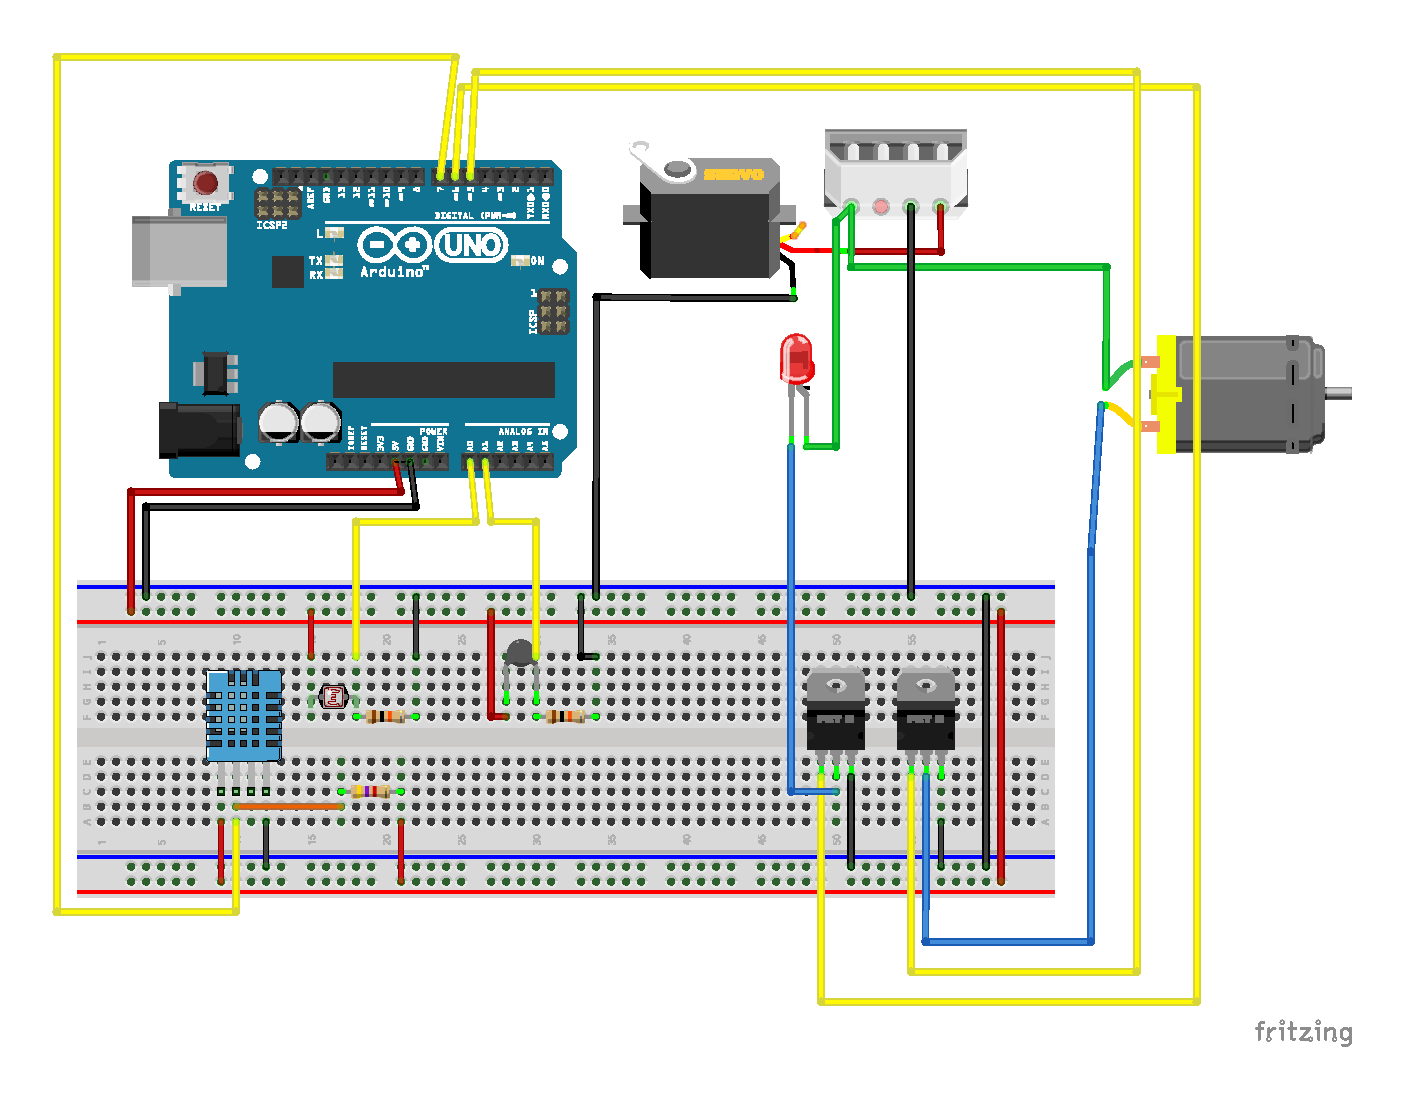
\includegraphics[width = 0.9\textwidth]{hardware.pdf}
            \end{figure}
		\end{frame}

		\begin{frame}{HAL - Présentation du Logiciel}
			Bla bla
		\end{frame}

		\begin{frame}{HAL - Notre contribution}
			Bla bla
		\end{frame}


\end{document}

